\documentclass{standalone}
\usepackage{tikz}
\usetikzlibrary{patterns, positioning}


\begin{document}
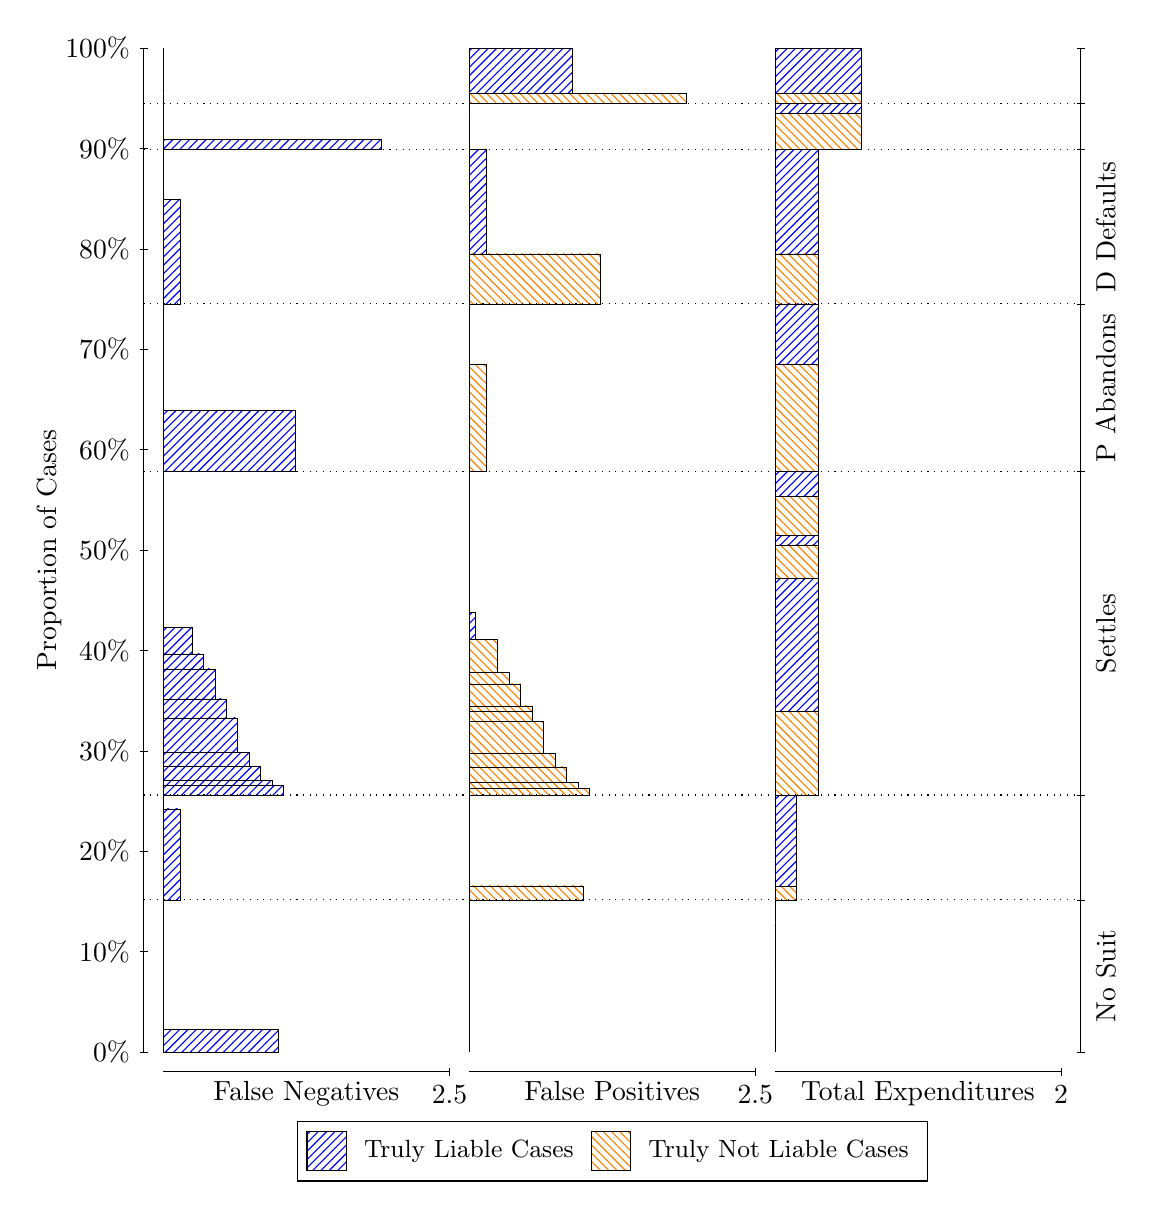
\begin{tikzpicture}
\draw[black, very thin] (1.5,1.75) -- (1.5,14.5);
\node[rotate=90, text=black, anchor=center] at (0.3, 8.125) {Proportion of Cases};
\draw[black, very thin] (1.45,1.75) -- (1.55,1.75);
\node[text=black, anchor=east] at (1.45, 1.75) {0\%};
\draw[black, very thin] (1.45,3.025) -- (1.55,3.025);
\node[text=black, anchor=east] at (1.45, 3.025) {10\%};
\draw[black, very thin] (1.45,4.3) -- (1.55,4.3);
\node[text=black, anchor=east] at (1.45, 4.3) {20\%};
\draw[black, very thin] (1.45,5.575) -- (1.55,5.575);
\node[text=black, anchor=east] at (1.45, 5.575) {30\%};
\draw[black, very thin] (1.45,6.85) -- (1.55,6.85);
\node[text=black, anchor=east] at (1.45, 6.85) {40\%};
\draw[black, very thin] (1.45,8.125) -- (1.55,8.125);
\node[text=black, anchor=east] at (1.45, 8.125) {50\%};
\draw[black, very thin] (1.45,9.4) -- (1.55,9.4);
\node[text=black, anchor=east] at (1.45, 9.4) {60\%};
\draw[black, very thin] (1.45,10.675) -- (1.55,10.675);
\node[text=black, anchor=east] at (1.45, 10.675) {70\%};
\draw[black, very thin] (1.45,11.95) -- (1.55,11.95);
\node[text=black, anchor=east] at (1.45, 11.95) {80\%};
\draw[black, very thin] (1.45,13.225) -- (1.55,13.225);
\node[text=black, anchor=east] at (1.45, 13.225) {90\%};
\draw[black, very thin] (1.45,14.5) -- (1.55,14.5);
\node[text=black, anchor=east] at (1.45, 14.5) {100\%};

\draw[black, very thin] (13.4,1.75) -- (13.4,14.5);
\draw[black, very thin] (13.35,1.75) -- (13.45,1.75);
\node[anchor=west] at (13.35, 1.75) {};
\draw[black, very thin] (13.35,3.6827) -- (13.45,3.6827);
\node[anchor=west] at (13.35, 3.6827) {};
\draw[black, very thin] (13.35,5.0135) -- (13.45,5.0135);
\node[anchor=west] at (13.35, 5.0135) {};
\draw[black, very thin] (13.35,9.1231) -- (13.45,9.1231);
\node[anchor=west] at (13.35, 9.1231) {};
\draw[black, very thin] (13.35,11.251) -- (13.45,11.251);
\node[anchor=west] at (13.35, 11.251) {};
\draw[black, very thin] (13.35,13.213) -- (13.45,13.213);
\node[anchor=west] at (13.35, 13.213) {};
\draw[black, very thin] (13.35,13.794) -- (13.45,13.794);
\node[anchor=west] at (13.35, 13.794) {};
\draw[black, very thin] (13.35,14.5) -- (13.45,14.5);
\node[anchor=west] at (13.35, 14.5) {};

\draw[black, very thin, pattern color=blue, pattern=north east lines] (1.75,1.75) rectangle (3.2033,2.0358);
\draw[black, very thin, pattern color=orange, pattern=north west lines] (1.75,2.0358) rectangle (1.75,3.6827);
\draw[black, very thin, pattern color=blue, pattern=north east lines] (1.75,3.6827) rectangle (1.968,4.8371);
\draw[black, very thin, pattern color=orange, pattern=north west lines] (1.75,4.8371) rectangle (1.75,5.0135);
\draw[black, very thin, pattern color=blue, pattern=north east lines] (1.75,5.0135) rectangle (3.276,5.1345);
\draw[black, very thin, pattern color=blue, pattern=north east lines] (1.75,5.1345) rectangle (3.1307,5.1999);
\draw[black, very thin, pattern color=blue, pattern=north east lines] (1.75,5.1999) rectangle (2.9853,5.3781);
\draw[black, very thin, pattern color=blue, pattern=north east lines] (1.75,5.3781) rectangle (2.84,5.5515);
\draw[black, very thin, pattern color=blue, pattern=north east lines] (1.75,5.5515) rectangle (2.6947,5.9928);
\draw[black, very thin, pattern color=blue, pattern=north east lines] (1.75,5.9928) rectangle (2.5493,6.2346);
\draw[black, very thin, pattern color=blue, pattern=north east lines] (1.75,6.2346) rectangle (2.404,6.615);
\draw[black, very thin, pattern color=blue, pattern=north east lines] (1.75,6.615) rectangle (2.2587,6.8044);
\draw[black, very thin, pattern color=blue, pattern=north east lines] (1.75,6.8044) rectangle (2.1133,7.1434);
\draw[black, very thin, pattern color=orange, pattern=north west lines] (1.75,7.1434) rectangle (1.75,9.1231);
\draw[black, very thin, pattern color=blue, pattern=north east lines] (1.75,9.1231) rectangle (3.4213,9.8944);
\draw[black, very thin, pattern color=orange, pattern=north west lines] (1.75,9.8944) rectangle (1.75,11.251);
\draw[black, very thin, pattern color=blue, pattern=north east lines] (1.75,11.251) rectangle (1.968,12.579);
\draw[black, very thin, pattern color=orange, pattern=north west lines] (1.75,12.579) rectangle (1.75,13.213);
\draw[black, very thin, pattern color=blue, pattern=north east lines] (1.75,13.213) rectangle (4.5113,13.34);
\draw[black, very thin, pattern color=orange, pattern=north west lines] (1.75,13.34) rectangle (1.75,13.794);
\draw[black, very thin, pattern color=orange, pattern=north west lines] (1.75,13.794) rectangle (1.75,13.921);
\draw[black, very thin, pattern color=blue, pattern=north east lines] (1.75,13.921) rectangle (1.75,14.5);
\draw[black, very thin, pattern color=orange, pattern=north west lines] (5.6333,1.75) rectangle (5.6333,3.3969);
\draw[black, very thin, pattern color=blue, pattern=north east lines] (5.6333,3.3969) rectangle (5.6333,3.6827);
\draw[black, very thin, pattern color=orange, pattern=north west lines] (5.6333,3.6827) rectangle (7.0867,3.8591);
\draw[black, very thin, pattern color=blue, pattern=north east lines] (5.6333,3.8591) rectangle (5.6333,5.0135);
\draw[black, very thin, pattern color=orange, pattern=north west lines] (5.6333,5.0135) rectangle (7.1593,5.0968);
\draw[black, very thin, pattern color=orange, pattern=north west lines] (5.6333,5.0968) rectangle (7.014,5.1734);
\draw[black, very thin, pattern color=orange, pattern=north west lines] (5.6333,5.1734) rectangle (6.8687,5.3711);
\draw[black, very thin, pattern color=orange, pattern=north west lines] (5.6333,5.3711) rectangle (6.7233,5.545);
\draw[black, very thin, pattern color=orange, pattern=north west lines] (5.6333,5.545) rectangle (6.578,5.9476);
\draw[black, very thin, pattern color=orange, pattern=north west lines] (5.6333,5.9476) rectangle (6.4327,6.0733);
\draw[black, very thin, pattern color=orange, pattern=north west lines] (5.6333,6.0733) rectangle (6.4327,6.1442);
\draw[black, very thin, pattern color=orange, pattern=north west lines] (5.6333,6.1442) rectangle (6.2873,6.4248);
\draw[black, very thin, pattern color=orange, pattern=north west lines] (5.6333,6.4248) rectangle (6.142,6.5702);
\draw[black, very thin, pattern color=orange, pattern=north west lines] (5.6333,6.5702) rectangle (5.9967,6.9932);
\draw[black, very thin, pattern color=blue, pattern=north east lines] (5.6333,6.9932) rectangle (5.706,7.3322);
\draw[black, very thin, pattern color=blue, pattern=north east lines] (5.6333,7.3322) rectangle (5.6333,9.1231);
\draw[black, very thin, pattern color=orange, pattern=north west lines] (5.6333,9.1231) rectangle (5.8513,10.48);
\draw[black, very thin, pattern color=blue, pattern=north east lines] (5.6333,10.48) rectangle (5.6333,11.251);
\draw[black, very thin, pattern color=orange, pattern=north west lines] (5.6333,11.251) rectangle (7.3047,11.886);
\draw[black, very thin, pattern color=blue, pattern=north east lines] (5.6333,11.886) rectangle (5.8513,13.213);
\draw[black, very thin, pattern color=orange, pattern=north west lines] (5.6333,13.213) rectangle (5.6333,13.667);
\draw[black, very thin, pattern color=blue, pattern=north east lines] (5.6333,13.667) rectangle (5.6333,13.794);
\draw[black, very thin, pattern color=orange, pattern=north west lines] (5.6333,13.794) rectangle (8.3947,13.921);
\draw[black, very thin, pattern color=blue, pattern=north east lines] (5.6333,13.921) rectangle (6.9413,14.5);
\draw[black, very thin, pattern color=orange, pattern=north west lines] (9.5167,1.75) rectangle (9.5167,3.3969);
\draw[black, very thin, pattern color=blue, pattern=north east lines] (9.5167,3.3969) rectangle (9.5167,3.6827);
\draw[black, very thin, pattern color=orange, pattern=north west lines] (9.5167,3.6827) rectangle (9.7892,3.8591);
\draw[black, very thin, pattern color=blue, pattern=north east lines] (9.5167,3.8591) rectangle (9.7892,5.0135);
\draw[black, very thin, pattern color=orange, pattern=north west lines] (9.5167,5.0135) rectangle (10.062,6.0733);
\draw[black, very thin, pattern color=blue, pattern=north east lines] (9.5167,6.0733) rectangle (10.062,7.7659);
\draw[black, very thin, pattern color=orange, pattern=north west lines] (9.5167,7.7659) rectangle (10.062,8.1888);
\draw[black, very thin, pattern color=blue, pattern=north east lines] (9.5167,8.1888) rectangle (10.062,8.3098);
\draw[black, very thin, pattern color=orange, pattern=north west lines] (9.5167,8.3098) rectangle (10.062,8.8067);
\draw[black, very thin, pattern color=blue, pattern=north east lines] (9.5167,8.8067) rectangle (10.062,9.1231);
\draw[black, very thin, pattern color=orange, pattern=north west lines] (9.5167,9.1231) rectangle (10.062,10.48);
\draw[black, very thin, pattern color=blue, pattern=north east lines] (9.5167,10.48) rectangle (10.062,11.251);
\draw[black, very thin, pattern color=orange, pattern=north west lines] (9.5167,11.251) rectangle (10.062,11.886);
\draw[black, very thin, pattern color=blue, pattern=north east lines] (9.5167,11.886) rectangle (10.062,13.213);
\draw[black, very thin, pattern color=orange, pattern=north west lines] (9.5167,13.213) rectangle (10.607,13.667);
\draw[black, very thin, pattern color=blue, pattern=north east lines] (9.5167,13.667) rectangle (10.607,13.794);
\draw[black, very thin, pattern color=orange, pattern=north west lines] (9.5167,13.794) rectangle (10.607,13.921);
\draw[black, very thin, pattern color=blue, pattern=north east lines] (9.5167,13.921) rectangle (10.607,14.5);
\draw[black, dotted] (1.5,3.6827) -- (13.4,3.6827);
\draw[black, dotted] (1.5,5.0135) -- (13.4,5.0135);
\draw[black, dotted] (1.5,9.1231) -- (13.4,9.1231);
\draw[black, dotted] (1.5,11.251) -- (13.4,11.251);
\draw[black, dotted] (1.5,13.213) -- (13.4,13.213);
\draw[black, dotted] (1.5,13.794) -- (13.4,13.794);
\draw[black, very thin] (1.75,1.5) -- (5.3833,1.5);
\node[text=black, anchor=north] at (3.5667, 1.5) {False Negatives};
\draw[black, very thin] (5.3833,1.45) -- (5.3833,1.55);
\node[text=black, anchor=north] at (5.3833, 1.45) {2.5};

\draw[black, very thin] (5.6333,1.5) -- (9.2667,1.5);
\node[text=black, anchor=north] at (7.45, 1.5) {False Positives};
\draw[black, very thin] (9.2667,1.45) -- (9.2667,1.55);
\node[text=black, anchor=north] at (9.2667, 1.45) {2.5};

\draw[black, very thin] (9.5167,1.5) -- (13.15,1.5);
\node[text=black, anchor=north] at (11.333, 1.5) {Total Expenditures};
\draw[black, very thin] (13.15,1.45) -- (13.15,1.55);
\node[text=black, anchor=north] at (13.15, 1.45) {2};

\node[text=black, centered, rotate=90] at (13.72, 2.7164) {No Suit};

\node[text=black, centered, rotate=90] at (13.72, 7.0683) {Settles};
\node[text=black, centered, rotate=90] at (13.72, 10.187) {P Abandons};
\node[text=black, centered, rotate=90] at (13.72, 12.232) {D Defaults};



\draw (7.449999999999999,1.5) node[draw=none] (baseCoordinate) {};
\begin{scope}[align=center]
        \matrix[scale=0.5, draw=black, below=0.5cm of baseCoordinate, nodes={draw}, column sep=0.1cm]{
            \node[rectangle, draw, minimum width=0.5cm, minimum height=0.5cm, pattern color=blue, pattern=north east lines] {}; &
            \node[draw=none, font=\small, text=black] (B) {Truly Liable Cases}; &
            \node[rectangle, draw, minimum width=0.5cm, minimum height=0.5cm, pattern color=orange, pattern=north west lines] {}; &
            \node[draw=none, font=\small, text=black] (B) {Truly Not Liable Cases}; \\
            };
\end{scope}

\end{tikzpicture}
\end{document}